\section*{Introduction}

The article that is the subject of this reproduction attempt was my first publication for which I provided code as supplementary material \cite{HinsenStructuralflexibilityproteins2008}. In computational biophysics, that was uncommon back in 2008, and unfortunately it remains the exception until today. The code consisted of two Python scripts plus instructions and was meant to help readers with applying the methods discussed in the article to different proteins, rather than ensure reproducibility which at that time I had never heard of. This explains why the supplied code does not reproduce the figures shown in the paper, but merely produces data files in plain text format, from which the plots were originally assembled by hand.

The work described in the original article was performed in summer 2007. The scripts make heavy use of two libraries of which I am the principal author: the Molecular Modeling Toolkit (MMTK) \cite{Hinsenmolecularmodelingtoolkit2000}, then at version 2.5, and ScientificPython, then at version 2.7. These two libraries, first published in 1997, are among the oldest scientific computing packages in the SciPy ecosystem. They were initially written on the basis of Numerical Python \cite{DuboisNumericalPython1996}, the original array package for Python that was published in 1995. With the transition to its successor NumPy \cite{OliphantguideNumPy2006}, initially released in 2006, I ported MMTK and ScientificPython to NumPy using its compatibility module called \texttt{oldnumeric}. This combination as used for the original work, but unfortunately I did not write down the exact version of NumPy. My instructions recommend ``Numerical Python 23.8.2 or NumPy 1.x'', which turned out to be overly optimistic: NumPy is still in the 1.x version range, but frequent breaking changes make it impossible to run my code with recent NumPy releases. In fact, with version~1.9 NumPy removed the \texttt{oldnumeric} interface, breaking all of my molecular simulation code. I had envisaged to port the code to the official NumPy API, but decided not to do so because of the high risk of introducing errors. There are in fact several subtle changes in the API, such as using the transpose of a matrix compared to the original Numeric API, which are easy to overlook because incorrect use yields an incorrect result but no error message. With the end of support for Python~2, there is longer any point in such a change: my code depends on unmaintained software anyway.

The remaining dependencies turned out to be less critical. netCDF, which my scripts use for data storage, was at version 3.4, but any more recent version can be substituted. Python itself, then at version 2.5, caused no problems either up to release 2.7. Python~3 is a very different language, with notably a very different C API layer, meaning that none of my code works with Python~3 and a port would indeed involve a significant amount of work because of the large number of extension modules in MMTK, most of which are C code hand-written for the C API of Python 1.4, long before Pyrex \cite{EwingPyrex} and then its fork Cython \cite{BehnelCythonBestBoth2011} introduced more convenient ways to write extension modules.

\section*{Reproduction}

The GitHub repository for this reproduction (\href{https://github.com/khinsen/rescience-ten-year-challenge-paper-3}) contains all the code, input data, and instructions for running the reproduction on a modern GNU/Linux system with the Guix package manager \cite{CourtesReproducibleUserControlledSoftware2015,WurmusPiGxreproduciblegenomics2018}. It also lists the exact version numbers of all the software involved in the reproduction. For the numerical calculations alone, i.e. excluding the less critical tasks of downloading files and generating plots, a total of 254 Guix package must be rebuilt identically to guarantee bit-for-bit reproduction of the results.

\subsection*{Finding the code and the input data}

The project-specific scripts are still available for download from the journal's Web site. All the dependencies have been available in public version-controlled repositories for many years. Obtaining the code is therefore not a problem.

The input data for reproducing the figures in the original paper consists of three protein structures from the Protein Data Bank (PDB) \cite{wwPDBconsortiumProteinDataBank2019}. The PDB updates its files from time to time. The file for a specifc entry is intended to represent the original data deposited by its authors, but may be modified to conform to newer versions of the file format, or to fix mistakes. There is thus no guarantee that a file downloaded today is the same as in 2008, but the scientific information it contains is supposed to stay the same. I am not aware of anyone ever reporting discrepancied in PDB entries over time.

\subsection*{Running the scripts using the Guix package manager}

My preferred software management tool for reproducible computations is the Guix package manager \cite{CourtesReproducibleUserControlledSoftware2015}, which permits the bit-for-bit reconstruction of software environments at any later time. All the required dependencies have already been packaged in Guix, but since Guix only started in 2012, and the Python ecosystem was added even later, the original software versions of 2008 are not available.

The two scripts are meant to be run in sequence, once for each protein structure and crystal size. The first script, \texttt{calculate\_crystal\_fluctuations.py}, computes the normal modes of the crystal and stores them in a netCDF file. The second script, \texttt{analyze\_crystal\_fluctuations.py} extracts the relevant data for the plots from the netCDF file and writes them to text files.

Using the dependencies as defined in Guix in January~2020 (more precisely: commit \texttt{7357b3d7a52eb5db1674012c50d308d792741c48}), the first script runs without any apparent problem, but the second one crashes with an error message. It is the result of a breaking change in NumPy which modified the rules for the conversion of sequence-like Python objects into arrays. This problem can be fixed by changing a single line of code; however, neither the diagnosis nor the correction are likely to be obvious to someone who is not intimately familiar with NumPy.

I explored the possibility of using an earlier NumPy release in order to run the scripts unmodified. From the release history that is available on NumPy's GitHub repository, it appears that release 1.0.4 was current at the time of submission of my paper in late 2007. Unfortunately, this NumPy release cannot be installed with Python 2.7 because NumPy is distributed with a modified version of the \texttt{distutils} package. \texttt{distutils}  reads a configuration file produced during the installation of Python, whose format has changed between Python 2.5 and 2.7. I briefly envisaged installing Python 2.5, but that would have required backporting the modifications made for Guix, which seemed an unreasonable effort for performing a simple test.

\subsection*{Reproducing the figures}

As explained in the introduction, my goal with publishing the code of my computations was to enable reuse, not reproducibility. The code therefore does not reproduce the full figures, which need to be re-generated by hand from the numerical output. I have limited myself to producing figures that are similar enough to the originals to convince the reader that the results have been reproduced correctly.

Figure~1 of the original publication does not contain any computed and has therefore not been reproduced. The data it shows comes directly from the Protein Data Bank.

Figures~2 and~3 of the original publication compare ``single molecule'' to ``crystal'' results for two proteins. Only the latter are computed by the scripts in the supplementary material, and are shown in Figs.~\ref{fig2} and~\ref{fig3}. The ``single molecule'' curves were obtained by a script that was not published, and which I have lost. It would not be difficult to replicate, but that is not the goal of this reproduction attempt.

\begin{figure}
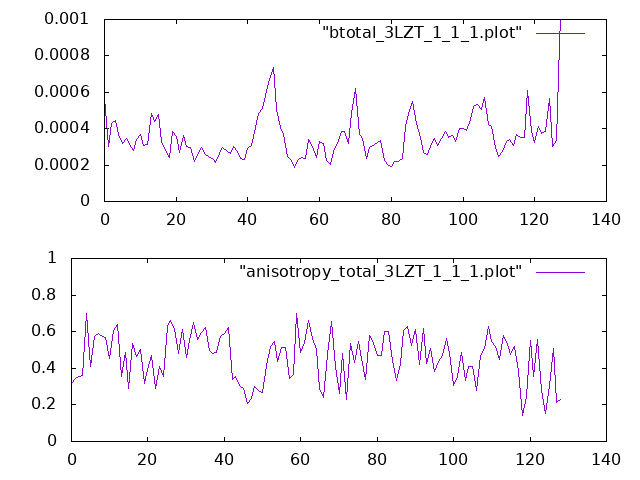
\includegraphics[width=.9\textwidth]{../reproduction/fig2.png}
\caption{Reproduction of Fig.~2 in the original publication.}
\label{fig2}
\end{figure}

\begin{figure}
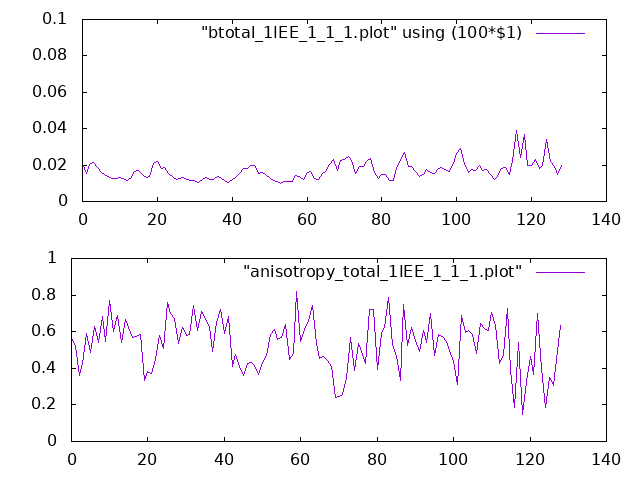
\includegraphics[width=.9\textwidth]{../reproduction/fig3.png}
\caption{Reproduction of Fig.~3 in the original publication.}
\label{fig3}
\end{figure}

Figure~4 of the original publication shows the dispersion relations for four different directions of wave propagation in the crystal. Unfortunately, the supplied scripts only produce a single file with points on the dispersion plots from all directions combined. The additional script required to separate these points by direction was not published and has been lost. The dashed lines labelled ``elastic medium'' were also computed by unpublished and lost scripts. Fig.~\ref{fig4} shows unconnected points that each lie on one of the drawn-out lines of the original Figure~4.
\begin{figure}
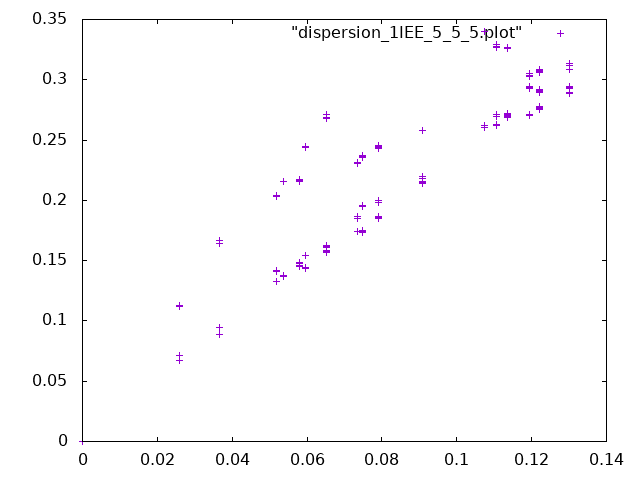
\includegraphics[width=.9\textwidth]{../reproduction/fig4.png}
\caption{Reproduction of Fig.~4 in the original publication.}
\label{fig4}
\end{figure}

Figure~5 of the original publication is reproduced almost entirely in Fig.~\ref{fig5}. One curve from the original plots, labelled ``extrapolation'', is missing because the script used for doing the extrapolation was not published and has been lost.
\begin{figure}
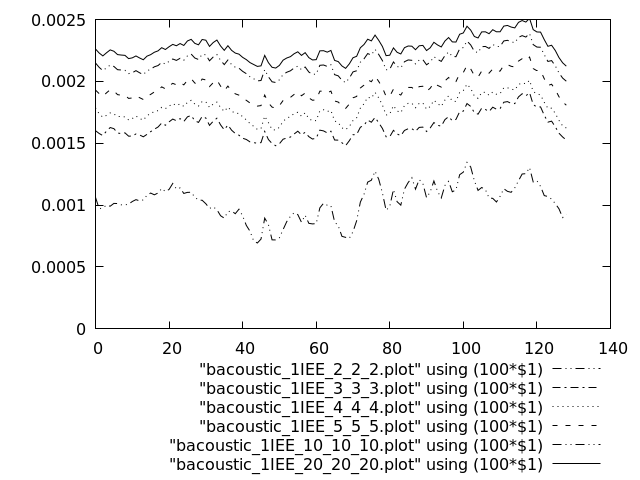
\includegraphics[width=.9\textwidth]{../reproduction/fig5a.png}
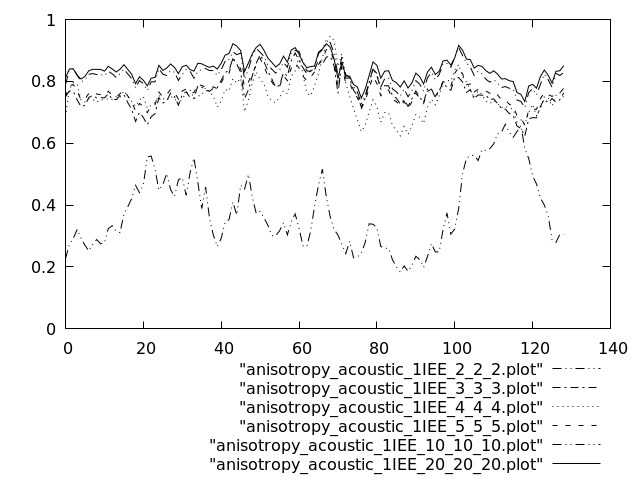
\includegraphics[width=.9\textwidth]{../reproduction/fig5b.png}
\caption{Reproduction of Fig.~5 in the original publication.}
\label{fig5}
\end{figure}

Finally, Figure~6 of the original publication has not been reproduced. It contains one curve each from Figs.~\ref{fig2} and~\ref{fig3}, combined with experimental data from the Protein Data Bank and a scaled curve using a scaling factor computed by yet another script that was not published and has been lost.

\section*{Conclusion}

The goal of this reproduction attempt was to answer three questions:
\begin{enumerate}
\item Can the code published in 2008 still be run today?
\item Does it produce results equivalent to those shown in the original figures?
\item Does the code fully reproduce the original results?
\end{enumerate}

My answers are
\begin{enumerate}
\item Yes, but only after modification.
\item Yes.
\item No, because not all the required code was published, and the unpublished code has been lost in the meantime.
\end{enumerate}

The obvious lesson for the future to draw from this exercise is the importance of publishing all the code, up to the automatic generation of figures and tables. Another regrettable omission I made in 2008 is not writing down the precise version numbers of all the code involved. It might have been useful in this case to know the precise version of NumPy used in the original work. In fact, my claim that the modification to a script was required as a consequence of a breaking change in NumPy is based merely on my memories and notes from other projects in which I had to make similar changes.

The final lesson would have to be drawn by a wider community of scientific software developers: breaking changes in widely used infrastructure code such as NumPy can cause a lot of damage in terms of lost reproducibility that may be difficult to diagnose and fix for someone else than the original authors. The open question that the scientific community has to figure out is where to place reproducibility on our scale of values, and for which time spans we consider it desirable. Structural biology is a methodologically mature domain of research, in which the main source of progress is not disruptive new methods, but incremental improvements of existing methods in the course of ongoing applications to biologically relevant systems. This is in fact the norm in science and technology \cite{Arthurnaturetechnologywhat2009}. In this context, my methodological work published in~2008 is by no means outdated. The last time I have referred to it myself (in so-far unpublished work) was in 2018. Reproducibility lifetimes of just a few years, which is the current state of the scientific Python ecosystem, are therefore problematic.
